
%     Copyright 2021, Abt Dávid Ottó

%         Szegedi Tudományegyetem
% Természettudományi és Informatikai Kar
%          Informatikai tanszék

% A szakdolgozathoz felhasználtam az alábbi linkeken található sablont:
% https://github.com/szledan/thesis-template

\documentclass[12pt,numbers=noenddot]{report}

\usepackage[a4paper]{geometry}
\usepackage{lmodern}			% Kijelölhető az összes karakter
\usepackage[utf8]{inputenc}		% Ékezetes szavak beviteléhez
\usepackage[hungarian]{babel}	% Magyar nyelv támogatása
\usepackage{fontspec}			% Fontok támogatása
\setmainfont{Nimbus Roman}		% FOSS Times New Roman alternatíva
\usepackage{titlesec}			% Fejlécben lévő cím margójának beállítására
\usepackage{fancyhdr}			% Fej- és láblécek személyreszabása
\usepackage{graphicx}			% Képek
\graphicspath{ {./img/} }
\usepackage{color}				% Színek
\usepackage{xcolor}				% -||-
\usepackage{subfig}
\usepackage{caption}
\captionsetup[figure]{labelsep=colon}
\usepackage{tikz}
\usepackage{float}				% Hogy az ábrák a helyükön maradjanak
\usepackage{wrapfig}			% Kép mellett folyó íráshoz
\usepackage{listings}			% Forráskódok
\usepackage{lastpage}			% Utolsó oldal száma
\usepackage[unicode]{hyperref}	% Linkek
\hypersetup{
	colorlinks,
	citecolor=black,
	filecolor=black,
	linkcolor=black,
	urlcolor=black
}
\usepackage[block=ragged]{biblatex}
\BiblatexHungarianWarningOff
\bibliography{cites}
\DeclareFieldFormat{urldate}{Látogatás:}

\usepackage{amsmath}

\usepackage{multicol}

\usepackage{amssymb} 

% Egyéni színek
\definecolor{codegreen}{rgb}{0,0.6,0}
\definecolor{codegray}{rgb}{0.5,0.5,0.5}
\definecolor{codepurple}{rgb}{0.58,0,0.82}
\definecolor{backcolour}{rgb}{0.95,0.95,0.92}

% Kódrészletek
\lstset{ %
	backgroundcolor=\color{backcolour},
	commentstyle=\color{codegreen},
	keywordstyle=\color{magenta},
	numberstyle=\tiny\color{codegray},
	stringstyle=\color{codepurple},
	basicstyle=\ttfamily\footnotesize,
	breakatwhitespace=false,
	breaklines=true,
	captionpos=b,
	keepspaces=true,
	numbers=left,
	numbersep=5pt,
	showspaces=false,
	showstringspaces=false,
	showtabs=false,
	tabsize=4,
	extendedchars=true
}

% Ábrák számozása
\renewcommand{\thefigure}{\arabic{chapter}.\arabic{figure}}
% Ábrák "ábra" felirata
\addto\captionsmagyar{\renewcommand{\figurename}{{\'a}bra}}

% Tartalomjegyzék elemeinek számozása:
\setcounter{tocdepth}{3}
\setcounter{secnumdepth}{3}

% Margók:
\voffset	-1in
\textwidth	150mm
\topmargin	15mm
\headheight	10mm
\headsep	5mm
\textheight	237mm

% A Word-ös 1.5-ös sorköznek ez felel meg
\linespread{1.25}

\begin{document}

\pagestyle{fancyplain}
\fancyhf{}
\renewcommand{\headrulewidth}{0pt}	% Eltűnteti a fejlécben lévő vonalat

\titleformat{\chapter}[display]
{\normalfont\huge\bfseries}{\thechapter. \chaptertitlename}{20pt}{\Huge}
\titlespacing*{\chapter}{0pt}{0pt}{40pt}

\newcommand{\szerzo}{Abt Dávid Ottó}
\newcommand{\cim}{Másodrendű sajátvektor centralitások vizsgálata}

%%%%%%%%%%%%%%%%%%%%%%%%%%%%%%%%%%%%%%%%%%%%%%%%%%%%%%%%%%%%%%%%%%%%%%%%%%%%%%%%
%% Elülső kötéstábla                                                          %%
%%%%%%%%%%%%%%%%%%%%%%%%%%%%%%%%%%%%%%%%%%%%%%%%%%%%%%%%%%%%%%%%%%%%%%%%%%%%%%%%

\newpage
\thispagestyle{empty}
\fancyfoot[C]{}	% Lábléc eltüntetése

\begin{center}

	\vspace*{2cm}

	{\Large\bf Szegedi Tudományegyetem}

	\vspace{.5cm}

	{\Large\bf Informatikai Intézet}

	\vspace*{8.5cm}

	{\Huge\bf SZAKDOLGOZAT}

	\vspace*{7cm}

	{\LARGE\bf \szerzo}

	\vspace*{.6cm}

	{\Large\bf 2022}

\end{center}

%%%%%%%%%%%%%%%%%%%%%%%%%%%%%%%%%%%%%%%%%%%%%%%%%%%%%%%%%%%%%%%%%%%%%%%%%%%%%%%%
%% Címlap                                                                     %%
%%%%%%%%%%%%%%%%%%%%%%%%%%%%%%%%%%%%%%%%%%%%%%%%%%%%%%%%%%%%%%%%%%%%%%%%%%%%%%%%

\newpage
\thispagestyle{plain}

\begin{center}
	\vspace*{.6cm}

	{\Large\bf Szegedi Tudományegyetem}

	\vspace{.5cm}

	{\Large\bf Informatikai Tanszékcsoport}

	\vspace*{3.5cm}

	{\LARGE\bf \cim}

	\vspace*{3.2cm}

	{\Large Szakdolgozat}

	\vspace*{3.5cm}

	\large
	\begin{tabular}{c@{\hspace{4cm}}c}
	\emph{Készítette:}						&\emph{Témavezető:}\\
	\textbf{\szerzo}						&\textbf{Dr. Vinkó Tamás}\\
	programtervező informatikus BSc				&egyetemi docens\\
	hallgató								&
	\end{tabular}

	\vspace*{3.5cm}

	\Large {
		Szeged\\
		\vspace{2mm}
		2022
	}
\end{center}

%%%%%%%%%%%%%%%%%%%%%%%%%%%%%%%%%%%%%%%%%%%%%%%%%%%%%%%%%%%%%%%%%%%%%%%%%%%%%%%%
%% Üres oldal                                                                 %%
%%%%%%%%%%%%%%%%%%%%%%%%%%%%%%%%%%%%%%%%%%%%%%%%%%%%%%%%%%%%%%%%%%%%%%%%%%%%%%%%

\newpage
\thispagestyle{plain}
\mbox{}

%%%%%%%%%%%%%%%%%%%%%%%%%%%%%%%%%%%%%%%%%%%%%%%%%%%%%%%%%%%%%%%%%%%%%%%%%%%%%%%%
%% Feladatkiírás                                                              %%
%%%%%%%%%%%%%%%%%%%%%%%%%%%%%%%%%%%%%%%%%%%%%%%%%%%%%%%%%%%%%%%%%%%%%%%%%%%%%%%%

\chapter*{Feladatkiírás}
\setcounter{page}{1}	% A lapszámláló újrainicializálása
\fancyfoot[R]{\thepage}
\addcontentsline{toc}{section}{Feladatkiírás}

Elterjedt hobbi az operációs rendszer, illetve kernel fejlesztése az olyan
programozók közt, akik szeretnének többet megtudni a számítógépek működéséről.
Ennek köszönhetően az interneten számos nyílt forráskódú hobbi operációs
rendszerrel, valamint az azok írásához felhasználható útmutatókkal
találkozhatunk. Sajnálatos módon ezen leírások nagy része elavult, túl
bonyolult, vagy nem elég részletes ahhoz, hogy egy kezdő bármit is megértsen
belőle, ezért elhatároztam, hogy megírok egy jól dokumentált, egyszerűen
használható és bővíthető operációs rendszert, és kialakítok hozzá egy gyorsan
felállítható fejlesztői környezetet, amelynek beüzemelése mindössze pár parancs.

\hfill \break
A feladat része, hogy az operációs rendszer rendelkezzen a legszükségszerűbb
alap funkciókkal, és tartalmazzon pár programot és/vagy játékot is.

%%%%%%%%%%%%%%%%%%%%%%%%%%%%%%%%%%%%%%%%%%%%%%%%%%%%%%%%%%%%%%%%%%%%%%%%%%%%%%%%
%% Tartalmi összefoglaló                                                      %%
%%%%%%%%%%%%%%%%%%%%%%%%%%%%%%%%%%%%%%%%%%%%%%%%%%%%%%%%%%%%%%%%%%%%%%%%%%%%%%%%

\chapter*{Tartalmi összefoglaló}
\addcontentsline{toc}{section}{Tartalmi összefoglaló}

\subsubsection*{A téma megnevezése}

\cim

\subsubsection*{A megadott feladat megfogalmazása}

A feladat egy olyan operációs rendszer megírása, amely bootolás után egy
egyszerű parancssori, illetve grafikus felhasználói felületet biztosít, és
emellett rendelkezik néhány programmal és játékkal is.

\subsubsection*{A megoldásmód}

Az egyszerűség kedvéért az összes program a kernelbe van "égetve", és
kernelszintű hozzáférése van, valamint néhány olyan elem megvalósításához,
amely nem része a feladatkiírásnak, és túl sok időbe telt volna egy működő
implementáció feltalálása, már létező nyílt forráskódú és szabad szoftverek
részeit portoltam le, vagy azok működési elvei alapján írtam meg a saját
implementációmat.

\subsubsection*{Alkalmazott eszközök, módszerek}

A fejlesztés a \textit{VSCodium} és \textit{Vim} szövegszerkesztők segítségével
zajlott C, C++ és 32-bites x86 assembly nyelven.
A szoftver fordítására a \textit{gcc, g++, gas} fordítókat, hibakereséshez
\textit{GDB}-t, virtualizációhoz pedig nagyrészt \textit{QEMU}-t, majd később az
\textit{Oracle VirtualBox}-ot használtam. A build folyamatokat a
\textit{GNU Make} szoftver segítségével automatizálam.

\subsubsection*{Elért eredmények}

Az operációs rendszerem sikeresen bootol virtuális gépeken, és a tesztelt
funkciók hiba nélkül működnek.

\subsubsection*{Kulcsszavak}

operációs rendszer, kernel, bootloader, GRUB, Intel, x86, QEMU, VirtualBox

%%%%%%%%%%%%%%%%%%%%%%%%%%%%%%%%%%%%%%%%%%%%%%%%%%%%%%%%%%%%%%%%%%%%%%%%%%%%%%%%
%% Tartalomjegyzék                                                            %%
%%%%%%%%%%%%%%%%%%%%%%%%%%%%%%%%%%%%%%%%%%%%%%%%%%%%%%%%%%%%%%%%%%%%%%%%%%%%%%%%

\renewcommand{\contentsname}{Tartalomjegyzék}
\tableofcontents

%%%%%%%%%%%%%%%%%%%%%%%%%%%%%%%%%%%%%%%%%%%%%%%%%%%%%%%%%%%%%%%%%%%%%%%%%%%%%%%%
%% Bevezetés                                                                  %%
%%%%%%%%%%%%%%%%%%%%%%%%%%%%%%%%%%%%%%%%%%%%%%%%%%%%%%%%%%%%%%%%%%%%%%%%%%%%%%%%

\chapter{Bevezetés}
\addcontentsline{toc}{section}{Bevezetés}
\pagestyle{fancy}

Manapság körbevesznek minket a számítógépek, és életünk nélkülözhetetlen részévé
váltak. Már gyerekkorom óta számítógépek közt nevelkedtem, mégis úgy éreztem,
hogy nem tudok róluk eleget. Gimnáziumi éveim alatt olvastam egy cikket egy
Terry Davis nevű programozóról, aki a saját operácios rendszerének
fejlesztésére szentelte az életét. Mivel mindig is érdekelt a számítógépek
működése, a cikk hatására elolvastam pár útmutatót arról, hogy hogyan írhanék
otthon egy saját operációs rendszert. Az egyik ilyen útmutatót követve el is
kezdtem a fejlesztést, azonban a nehézségek miatt hamar feladtam.

Egészen az egyetem második évéig nem rendelkeztem sem elegendő tudással,
kitartással, sem pedig idővel egy ekkora méretű projekthez. Ekkor a nyári
szünetben kezdtem újra a projektet, és a szakdolgozattal beadott "végleges"
verzió befejezéséig csaknem másfél év telt el, ezalatt folyamatosan
fejlesztettem.

Az operációs rendszeremet második kutyám (Rex) után RexOS-re kereszteltem. A
fejlesztés és a tanulás során azt vettem észre, hogy a legtöbb operációs
rendszerek, illetve kernelek fejlesztéséhez való útmutató elavult információkkal
szolgál, vagy nehezen érthető egy kezdő számára, és sokszor a kódrészletek
hibásak / hiányosak, vagy pedig egyáltalán nincs is kódrészlet, ami segítené
egy-egy folyamat működésének megértését.
Ezek a nehézségek vettek rá, hogy a projektemben ügyeljek a kód átláthatóságára
és arra, hogy jól legyen dokumentálva, illetve hogy mindenki számára elérhető
legyen, ezzel segítve a hobbi operációs rendszerek fejlesztőit.

A 32-bites Intel architektúra mellett döntöttem, mert ehhez találtam a legtöbb
forrásanyagot, így a fejlesztése könnyebbnek bizonyult, mint egy 64-bites
operációs rendszeré. Eredetileg az is szerepelt a céljaim közt, hogy
lehessen valós hardveren futtatni, azonban erről lemondtam, amikor megtudtam,
hogy a mai számítógépek nem támogatják a VGA mode 3-at, amit az operációs
rendszerem a tartalom megjelenítésére használ, valamint a VESA VBE-t támogató
hardware is egyre ritkább.

%%%%%%%%%%%%%%%%%%%%%%%%%%%%%%%%%%%%%%%%%%%%%%%%%%%%%%%%%%%%%%%%%%%%%%%%%%%%%%%%
%% Alapfogalmak                                                               %%
%%%%%%%%%%%%%%%%%%%%%%%%%%%%%%%%%%%%%%%%%%%%%%%%%%%%%%%%%%%%%%%%%%%%%%%%%%%%%%%%

\chapter{Alapfogalmak}
\addcontentsline{toc}{section}{Bevezetés}
\pagestyle{fancy}

\section{Gráf}

Egy gráf definiálható egy $G=(V,E)$ párként, ahol V a gráf csúcsainak, E az 
éleinek halmaza. Az E halmaz V-beli elempárokat tartalmaz. 
($E \subseteq V \times V$)

Ez a matematikai struktúra alkalmas különböző entitások közti bináris kapcsolatok 
tárolására. Ezek lehetnek akár egy szociális médiai platform felhasználói közti 
ismerettségek, vagy egy internetes enciklopédia kulcsszavai közti összefüggések. 
A gráfok ezen tulajdonságát használja ki például a \textit{neo4j} nevű gráf 
adatbázis kezelő rendszer is.

\section{Mátrix}
A mátrix egy kétdimenziós listaként képzelhető el, ami nem csupán egy $m * n$ 
elemet tároló struktúra, hanem az elemek elhelyezkedésének köszönhetően jóval 
több információt tárol mint egy $m * n$ elemű halmaz.

\section{Gráf ábrázolások, mátrix}
A gráfokat ábrázolására a két legnépszerűbb adatszerkezet a szomszédsági lista, 
illetve a szomszédsági mátrix.

A másodrendű sajátvektor centralitások vizsgálatához a szomszédsági mátrixokat 
fogjuk használni, mivel mátrixokon jóval könnyebb az ezekhez szükséges 
műveleteket elvégezni mint láncolt listákon.

A szomszédsági mátrix egy $n \times n$-es mátrix, ahol $n$ a gráf csúcsainak 
száma. Az $m$-edik sor $n$-edik eleme megadja, hogy a gráf $m$-edik és 
$n$-edig csúcsa közt vezet-e él.


\pagebreak

\section{Sajátérték, sajátvektor}
A mátrixokat felfoghatjuk egy geometriai transzformációként amit egy vektoron 
végzünk el. Például az $\textbf{A}$ mátrix a $\vec{v}$ vektort az alábbiak 
szerint módosítja:

$$
\textbf{A} \vec{v} = \vec{w}
$$

$$
{
	\begin{bmatrix}
		a & b \\
		c & d \\
	\end{bmatrix}
}
{
	\begin{bmatrix}
		x \\
		y \\
	\end{bmatrix}
}
=
{
	\begin{bmatrix}
		a*x+b*y \\
		c*x+d*y \\
	\end{bmatrix}
}
$$

\vspace{1cm}

A transzformáció irányát és mértékét a sajátvektor és a sajátérték jellemzi.
Definíció szerint $A$ mátrix $v$ sajátétvektora és $\lambda$ sajátértéke 
közt az összefüggés: $$A \lambda = v \lambda$$


\section{Centralitás}
A gráfok atomi tulajdonságain (pl.: van-e él két csúcs között) kívül sok 
értékes információ kinyerhető különböző metrikákkal. Például a csúcsok 
"fontosságának" egy kimutatására szolgálnak a centralitások, amik egy sorrendet 
képeznek a gráf pontjai közt. 

A legegyszerűbb centralitás a fokszám centralitás, ami az adott csúcs fokszáma 
szerint képez sorrendet.


\noindent
\begin{minipage}[c]{0.4\linewidth}

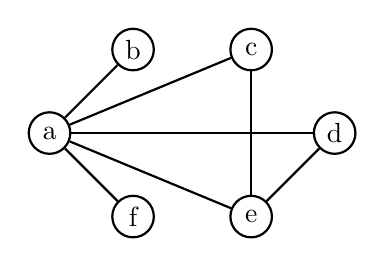
\begin{tikzpicture}[node distance=15mm, inner sep=0pt, minimum size=15pt, 
		thick, main/.style = {draw, circle}]
	\node[main] (1) {a};
	\node[main] (2) [above right of=1] {b};
	\node[main] (3) [right of=2] {c}; 
	\node[main] (4) [below right of=3] {d};
	\node[main] (5) [below left of=4] {e}; 
	\node[main] (6) [left of=5] {f};
	\draw (1) -- (2);
	\draw (1) -- (3);
	\draw (1) -- (4);
	\draw (1) -- (5);
	\draw (1) -- (6);
	\draw (3) -- (5);
	\draw (4) -- (5);
\end{tikzpicture}

\end{minipage}
% \columnbreak
\noindent
\begin{minipage}[c]{0.2\linewidth}

\hspace{0.5cm}
$\rightarrow$

\end{minipage}
% \columnbreak
\begin{minipage}[c]{0.2\linewidth}

\begin{align}
	\begin{bmatrix}
		deg(a)\\
		deg(b)\\
		deg(c)\\
		deg(d)\\
		deg(e)\\
		deg(f)
	\end{bmatrix}
	=
	\begin{bmatrix}
		5\\
		1\\
		2\\
		2\\
		3\\
		1
	\end{bmatrix}
\end{align}

\end{minipage}

\vspace{0.5cm}

A ábrán szereplő 6 pontú gráfhoz egy 6 hosszúságú vektort rendelt, 
melynek elemei az egyes csúcsok fokszámával egyeznek meg.

A fokszám centralitás kiszamítható gráfot leíró $n \times n$ szomszédsági 
mátrix valamint egy $n$ elemű, egyesekből álló vektor szorzataként:

\begin{align}
	\begin{bmatrix}
		0 & 1 & 1 & 1 & 1 & 1 \\
		1 & 0 & 0 & 0 & 0 & 0 \\
		1 & 0 & 0 & 0 & 1 & 0 \\
		1 & 0 & 0 & 0 & 1 & 0 \\
		1 & 0 & 1 & 1 & 0 & 0 \\
		1 & 0 & 0 & 0 & 0 & 0 \\
	\end{bmatrix}
	*
	\begin{bmatrix}
		1\\
		1\\
		1\\
		1\\
		1\\
		1
	\end{bmatrix}
	=
	\begin{bmatrix}
		5\\
		1\\
		2\\
		2\\
		3\\
		1
	\end{bmatrix}
\end{align}


\section{Tenzor}

Egy skalár egy szám, egy $n$ elemű vektort $n$ rendezett érték, egy 
$n \times m$-es mátrix $n*m$ számstruktúra tárolására képes. 
Ezeket a matematikai fogalmakat általánosíthatjuk a tenzorokkal. 
A skalár egy nullad-, a vektor egy első-, a mátrix pedig egy másodrendű tenzornak 
tekinthatő.

Amiért igazán fontos behozni a tenzor fogalmát az az, hogy nem állunk meg a 
másodrendűségnél, léteznek magasabb rendű tenzorok is. Például egy 
$3 \times 3 \times 3$-as tenzor 27 elemből áll, és felfogható egy három 
dimenziós tömbként.


%%%%%%%%%%%%%%%%%%%%%%%%%%%%%%%%%%%%%%%%%%%%%%%%%%%%%%%%%%%%%%%%%%%%%%%%%%%%%%%%
%% Másodrendű sajátvektor centralitások                                       %%
%%%%%%%%%%%%%%%%%%%%%%%%%%%%%%%%%%%%%%%%%%%%%%%%%%%%%%%%%%%%%%%%%%%%%%%%%%%%%%%%

\chapter{Másodrendű sajátvektor centralitások}


\section{Elsőrendű centralitás}

A korábban látott fokszám centralitás egy elsőrendő centralitás volt,
mivel fokszám az adott csúcshoz kapcsolódó élek számát jelenti,
egy él pedig két csúcs között teremt kapcsolatot. 

Az elsőrendű centralitások kiszámításához elég volt egy mátrixszorzást 
végrehajtani egy vektoron, hiszen a mátrix felfogható egy kétdimenziós tömbként
is, aminek az $A[i][j]$-edig eleme jellemzi az összefüggést az $i$-edik és 
$j$-edik csúcs között.


\section{Másodrendű centralitás}

A másodrendű centralitás ezzel szemben csúcshármasok közti kapcsolatok alapján 
fogja jellemezni a gráfot. Három-három csúcs viszonyának tárolására a mátrixok 
nem elegendőek, harmadrendű tenzorok viszont igen.
Ezt fogjuk felhasználni a következőkben.


\section{Általános sajátvektor modell}

A másodrendű centralitások számításához egy operátorra lesz szükség, 
amely végrehajtra a megfelelő leképezést.

Egy \boldmath{$T$}\unboldmath $\in \mathbb{R}^{n \times n \times n}$ 
tenzorhoz és egy $p$ valós paraméterhez definiálunk egy \boldmath{$T_p$}
\unboldmath $: \mathbb{R}^n \rightarrow \mathbb{R}^n$ operátort,
ami egy $n$ elemű vektorhoz egy $n$ elemű vektort rendel. 
Az eredményvektor $i$-edik elemét a következőképp kaphatjuk meg:

$$\boldsymbol{T_p}(\boldsymbol{x})_i = \sum_{j,k=1}^n \boldsymbol{T}_{ijk} 
\mu_p(x_j,x_k)$$

ahol $\mu_p(x_j,x_k)$ a hatványközép, azaz:

$$\mu_p(x_j,x_k) = \left(\frac{|a|^p+|b|^p}{2}\right)^{1/p}$$


Ahhoz, hogy hatékonyan vizsgálatokat tudjunk végezni a különböző 
centralitásokon szükségünk lesz egy egységes kiszámítási módra.

Legyen $\alpha \in \mathbb{R}: 0 \leq \alpha \leq 1$ skalár, ami az első- 
és másodrendűség lineáris kombinációjának az arányát adja meg,
illetve legyen $M \in \mathbb{R}^{n \times n}$ nemnegatív elemekből álló, 
a gráfhoz tartozó négyzetes mátrix, valamint $\boldsymbol{T} \in 
\mathbb{R}^{n \times n \times n}$ szintén nemnegatív elemegkből álló, 
gráfot jellemző tenzor. Ekkor definiálhatunk egy $\mathcal{M}: 
\mathbb{R}^n \rightarrow \mathbb{R}^n$ operátort, hogy

$$\mathcal{M}(\boldsymbol{x}) = \alpha M \boldsymbol{x} + (1-\alpha) 
\boldsymbol{T}_p(\boldsymbol{x})$$

\noindent
Ekkor az első- és a másodrendű centralitás $i$-edik csúcsbeli értéke $x_i 
\geq 0$ ahol x kielégíti a sajátérték problémát:
$$\mathcal{M}(\boldsymbol{x}) = \lambda \boldsymbol{x}$$

\noindent
$\alpha$ megfelelő megválasztásával kiszámíhatjuk csak az elsőrendű 
centrailtás értéket $(\alpha = 1)$, vagy csak a másodrendű centralitás 
értéket $(\alpha = 0)$, illetve a kettő súlyozott kombinációját is.


\section{$M$ és $\boldsymbol{T}$ megválasztása}

Az $M$ mátrix az elsőrendű összetevője, tehát valamilyen elsőrendű 
információt kellene elkódolnia. 
Erre egy kézenfekvő lehetőség a szomszédsági mátrix.

A fontosabb szerepet pedig a $\boldsymbol{T}$ tenzor tölti be, hiszen ez 
tartalmazza a vizsgálandó másodrendű kapcsolatokat.

\subsection*{Bináris háromszögtenzor}

TODO

\subsection*{``Random séta'' háromszögtenzor}

TODO

\subsection*{Klaszterező-együttható háromszögtenzor}

TODO

\subsection*{Local closure triangle tensor (?)}

TODO


%%%%%%%%%%%%%%%%%%%%%%%%%%%%%%%%%%%%%%%%%%%%%%%%%%%%%%%%%%%%%%%%%%%%%%%%%%%%%%%%
%% Implementáció                                                              %%
%%%%%%%%%%%%%%%%%%%%%%%%%%%%%%%%%%%%%%%%%%%%%%%%%%%%%%%%%%%%%%%%%%%%%%%%%%%%%%%%

\chapter{Implementáció}

\section{Fejlesztői környezet}

A programot GNU/Linux operácios rendszer alatt VSCodium-ban fejlesztettem 
(Visual Studio Code nyílt forráskódú és szabad változa). A python nyelvet 
választottam, ami egy széles körben elterjedt szkriptnyelv, egyszerű 
szintaxissal, és sokrétű matematikai függvénykönyvtárakkal rendelkezik,
így a célnak tökéletesen megfelel.

A NetworkX a használt csomagok közül a legfontosabb, a gráfok beolvasását,
kezelését, illetve a rajtuk elvégzett műveleteket is támogatja. Ezen kívül
említésre méltó még a NumPy és a Pandas, amiket mátrixműveletek kiszámítására
használtam, valamint az argparse, amit parancssori argumentumok beolvasásában 
segített, illetve a Matplotlib, amivel az eredményeket kirajzoltattam.

\section{A program magja}

Ahhoz, hogy gráfok centralitását összehasonlítsuk, először ki kell tudni szamolni őket.
Az első lépés ennek az implementációja volt. Bemenetként egy gráfot kapunk, és az elvárt kimenet a 
$\mathcal{M}(\boldsymbol{x}) = \lambda \boldsymbol{x}$
egyenlet egy közelítő megoldása. 

Az egyenlet kiszámításához egy iterációs módszerre lesz szükségünk, a hatványmódszerre.
Ez az eljárás iteratív lépések segítségével a legnagyobb abszolútértékű sajátértékhez
és a hozzá tartozó sajátvektorhoz ad közelítő megoldást. 
Az algoritmus alapja ez az iteráció:
$$\boldsymbol{y}^{(k)} = A \boldsymbol{x}^{(k)}$$
$$\boldsymbol{x}^{(k+1)} = \frac{\boldsymbol{y}^{(k)}}{||\boldsymbol{y}^{(k)}||}$$

ahol az első egyenlet egy mátrix-vektor szorzás, a második pedig ennek a részeredménynek a normált értékét adja meg.
A kiinudlási ($\boldsymbol{x}^{(0)}$) vektor nem lehet merőleges a legnagyobb abszolútértékű sajátértékhez tartozó sajátvektorra.

\pagebreak

A mi esetünkben ez a következőképpen néz ki:

$$\boldsymbol{y}^{(k)} = \mathcal{M}(\boldsymbol{x})$$
$$\boldsymbol{x}^{(k+1)} = \frac{\boldsymbol{y}^{(k)}}{||\boldsymbol{y}^{(k)}||}$$

vagyis

$$\boldsymbol{y}^{(k)} = \alpha M \boldsymbol{x} + (1-\alpha) \boldsymbol{T}_p(\boldsymbol{x})$$
$$\boldsymbol{x}^{(k+1)} = \frac{\boldsymbol{y}^{(k)}}{||\boldsymbol{y}^{(k)}||}$$


\section{Az egyenlet paraméterei}

A kiszámítás előtt szükségünk lesz az $\alpha$-ra, az $M$-re, illetve $\boldsymbol{T_p}$-re, és a hozzá szükséges tenzorra.
Alfa egyszerű skalár paraméter, $M$-et, mint szomszédsági mátrixot pedig megkaphatjuk 
a NetworkX \texttt{adjacency\_matrix} nevű függvényével.

A tenzorok előállítását saját függvényekkel oldottam meg. 
Az input itt is egy gráf (NetworkX-es \texttt{Graph} típusban eltárolva),
és hátrom egymásba ágyazott for ciklus tölti fel a háromdimenziós tömbként tárolt tenzorokat.
Ezeke a függvények felépítésükben nagyban hasonlítanak, egyedül a tenzor értékét adó logika tér el.
Itt említést érdemel a NumPy csomag \texttt{ndarray, multiply, matmul} és \texttt{ones} függvényei,
amik sok forciklus megírását spórolták meg, ezzel rövidebbé, és átláthatóbbá téve a kódot.

A $\boldsymbol{T_p}$ operátornak egy háromparaméteres függvényt írtam, ami a tenzort, 
az $\boldsymbol{x}$ vektort, illetve $p$-t kapja inputként. 
A vektort itt egy hagyományos pyhton-os listaként kezeltem.

Még egy fontos paraméter, ami az egyenletben nincs explicit jelölve, az az iterációk száma.
Mivel iterációs módszerről beszélünk, így meg kell adni egy egész értéket is, 
hogy hány iteráció után szeretnénk visszatérni az eredménnyel. Minél tovább iterálunk,
annál pontosabb eredményt kapunk, azonban annál több erőforrást és időt vesz igénybe a program.

$\boldsymbol{x}$ kezdeti értékét eleinte egy random $n$ hosszúságú vektorra állítottam be,
aztán a determinisztikus műkösés miatt áttértem az egyesekből álló vektorra, így 
könnyebb volt a későbbiekben ellenőrizni a program helyességét.


\section{Teszt adatok}

A NetworkX a gráfokkal kapcsolatos függvényeken és eljárásokon kívül 
tartalmaz néhány gráfot is, például Zachary karate klubjának a gráfját.
Én is ezt használom a teszteléshez, illetve a program ezzel számol 
alapértelmezett gráfként, ha nem adunk meg mást.

Egyéb gráfok beszerzésére a \href{https://networkrepository.com/index.php}{Netwrok Repository}
oldalt használtam, ahool több ezer gráf áll rendelkezésre ingyenesen. 
Igyekeztem kisebb fokszámú $(|V|<100)$, de nem triviális gráfokat keresni.


\section{A keretprogram}
A szoftvert egy mérésre, kísérletezésre alkalmas eszközként képzeltem el,
amiben a matematikai számításokon van a hangsúly, nem pedig a felhasználói felületen.
Így a Unix filozófiához hűen egyszerű parancssori alkalmazásban gondolkoztam,
ami ``egy dolgot csinál, de azt jól csinálja''.

A program fejlesztésének első fázisában probléma volt, hogy az aktuális haladást
mindig ki akartam próbálni, esetleg az eredményeket képeken ábrázolni, és aztán
változtatni rajta, újra kipróbálni. Erre kézenfekvő megoldás volt, hogy 
az alkalmazásnak a számításhoz szükséges benemeneti paramétereken kívül 
meg lehessen adni, hogy milyen funkciót végezzen el.
Így ha valami újfajta mérést szerettem volna leimplementálni, akkor elég volt
létrehozni neki egy új funkciót, amit a helyes paraméterezés esetén végrehajt.




%%%%%%%%%%%%%%%%%%%%%%%%%%%%%%%%%%%%%%%%%%%%%%%%%%%%%%%%%%%%%%%%%%%%%%%%%%%%%%%%
%% Konklúzió                                                                  %%
%%%%%%%%%%%%%%%%%%%%%%%%%%%%%%%%%%%%%%%%%%%%%%%%%%%%%%%%%%%%%%%%%%%%%%%%%%%%%%%%

\chapter{Konklúzió}

A QEMU-ban, illetve VirtualBox-ban végrehajtott tesztelés összességében sikerrel
zajlott. Az alábbiakban részletezem a tesztelt funkciókat, és a kapott
eredményt.

\hfill \break
Végrehajtott tesztek:

\begin{enumerate}
	\item Bootolás QEMU-ban és VirtualBox-ban- sikeres
	\item Megszakítások - működnek
	\item PCI - kilistázza az összes PCI sínnel csatlakoztatott perifériát
	\item Fájlrendszer - felismeri a FAT32-es elsődleges partíciókat, és
	működik a fájlok tartalmának olvasása is
	\item Hálózat (VirtualBox) - működik a kommunikáció a számítógépen nyitott
	netcat-tel, illetve Android eszközön futtatott Debianon lévő netcat-tel is
	\item Soros port (QEMU) - bootoláskor kiírja a boot logot a standard
	outputra, illetve standard inputra bevitt karakterek megjelennek RexOS-en
	\item Párhuzamos port (QEMU) - kiírja a kívánt szöveget
	\item Játékok - hiba nélkül működnek
\end{enumerate}

\noindent Nem lett letesztelve:

\begin{enumerate}
	\item Hálózat (QEMU)
	\item Soros, illetve párhuzamos port (VirtualBox)
	\item Valós hardveren bootolás
\end{enumerate}

\noindent Az operációs rendszerem fejlesztése során rengeteg új információt,
tudást sajátítottam el, és sikerült közelebb kerülnöm a számítógépek működésének
megértéséhez.

%%%%%%%%%%%%%%%%%%%%%%%%%%%%%%%%%%%%%%%%%%%%%%%%%%%%%%%%%%%%%%%%%%%%%%%%%%%%%%%%
%% Irodalomjegyzék                                                            %%
%%%%%%%%%%%%%%%%%%%%%%%%%%%%%%%%%%%%%%%%%%%%%%%%%%%%%%%%%%%%%%%%%%%%%%%%%%%%%%%%

\clearpage
\phantomsection
\addcontentsline{toc}{section}{Irodalom}

\printbibliography

%%%%%%%%%%%%%%%%%%%%%%%%%%%%%%%%%%%%%%%%%%%%%%%%%%%%%%%%%%%%%%%%%%%%%%%%%%%%%%%%
%% Nyilatkozat                                                                %%
%%%%%%%%%%%%%%%%%%%%%%%%%%%%%%%%%%%%%%%%%%%%%%%%%%%%%%%%%%%%%%%%%%%%%%%%%%%%%%%%

\chapter*{Nyilatkozat}
\addcontentsline{toc}{section}{Nyilatkozat}

Alulírott \szerzo, Programtervező Informatikus hallgató, kijelentem,
hogy a dolgozatomat a Szegedi Tudományegyetem, Informatikai Tanszékcsoport
Szoftverfejlesztési Tanszékén készítettem, alapszakos diploma megszerzése
érdekében.

\hfill \break
Kijelentem, hogy a dolgozatot más szakon korábban nem védtem meg, saját munkám
eredménye, és csak a hivatkozott forrásokat (szakirodalom, eszközök, stb.)
használtam fel.

\hfill \break
Tudomásul veszem, hogy szakdolgozatomat a Szegedi Tudományegyetem
Informatikai Tanszékcsoport könyvtárában, a helyben olvasható könyvek között
helyezik el.

\vspace*{2cm}

\begin{tabular}{lc}
Szeged, \today
\hspace{2cm} & \makebox[6cm]{\dotfill} \\
& aláírás \\
\end{tabular}

%%%%%%%%%%%%%%%%%%%%%%%%%%%%%%%%%%%%%%%%%%%%%%%%%%%%%%%%%%%%%%%%%%%%%%%%%%%%%%%%
%% Köszönetnyilvánítás                                                        %%
%%%%%%%%%%%%%%%%%%%%%%%%%%%%%%%%%%%%%%%%%%%%%%%%%%%%%%%%%%%%%%%%%%%%%%%%%%%%%%%%

\chapter*{Köszönetnyilvánítás}
\addcontentsline{toc}{section}{Köszönetnyilvánítás}

Szeretném megköszönni a hasznos ismertetőket és kódrészleteket az
\textbf{OSDev wiki szerkesztőinek}, illetve az \textbf{OSDev Discord
szerver tagjainak} útbaigazításait, \textbf{James Molloynak} a kiváló
leírásokkal teli weboldalát, az érthető és szórakoztató
\textit{Write your own Operating System} c. videósorozatot pedig
\textbf{Viktor Engelmannak}. Ez a YouTube videósorozat rengeteget segített nekem
a fejlődésben és az operációs rendszerek működésének megértésében. Egyúttal
szeretném megköszönni a segítségét minden ismerősömnek, aki részt vett az
operációs rendszerem tesztelésben.

\end{document}
